
{\color{brown}\textbf{Ejemplo 3}}
En una tienda se venden rollos de papel higiénico. Cada rollo cuesta 2 dólares, pero hay la siguiente oferta:
Lleva 3 rollos de papel higiénico y paga solo 2.
Carlos compra 20 rollos del papel higiénico en oferta en esa tienda.\\
\textbf{¿Es correcto afirmar que pagó 40 dólares?}\\

Para resolver este problema utilizaremos una tabla de valores como la siguiente:


% \begin{tikzpicture}
%   \matrix[matrix of math nodes,draw, column sep=1em,row sep=.5mm] (mx) {
%     3 & 2 & $2\times2=4 $ \\
%     4 & 3 & $2\times3=6 $ \\
%     5 & 4 & $2\times4=8 $ \\
%     6 & 4 & $2\times4=8 $ \\
%     7 & 5 & $2\times5=10$ \\
%     8 & 6 & $2\times6=12$ \\
%     9 & 6 & $2\times6=12$ \\
%   };
%   \path[->,shorten >=2pt]
%   \foreach \from/\to in {1/9} {
%       ([yshift=2mm]mx-1-\from.north) edge[bend left]
%       node[above] {$\scriptstyle+1$} ([yshift=2mm]mx-1-\to.north)
%       ([yshift=-2.5mm]mx-2-\from.south) edge[bend right]
%       node[below] {$\scriptstyle+2$} ([yshift=-2.5mm]mx-2-\to.south)
%     };
%   \foreach \x in {2,...,6}{
%       \draw ([xshift=-0.5em]mx.north west -| mx-1-\x.west) -- ([xshift=-0.5em]mx.south west -| mx-1-\x.west);
%     };
%   \draw (mx.west) -- (mx.east);
% \end{tikzpicture}
% % \end{table}


\begin{figure}[H]
    \centering
    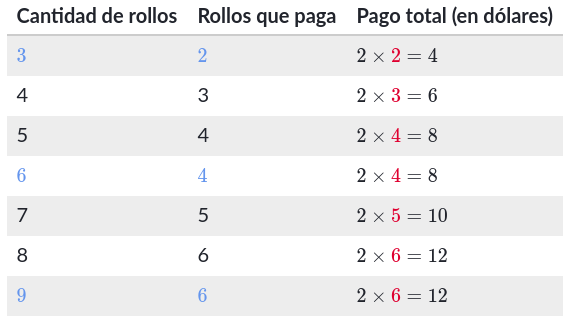
\includegraphics[width=0.5\textwidth]{./Unidad 2/Images/tableS8L102.png}
\end{figure}

Observamos que, si la cantidad de rollos es un múltiplo de 3, se cumple una relación proporcional
directa entre dicha cantidad y los rollos que deberá pagar. Como Carlos compra 20 rollos, podemos
observar que el múltiplo de 3 más cercano a 20 es 18. Así obtendremos la cantidad de rollos a pagar
luego de aplicar la oferta.\\

\begin{figure}[H]
    \centering
    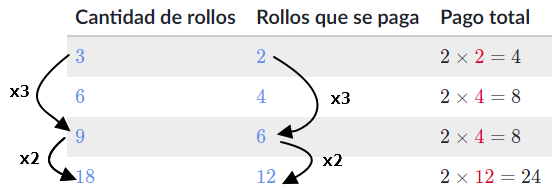
\includegraphics[width=0.5\textwidth]{./Unidad 2/Images/tableS8L101.png}
\end{figure}

Gracias a la tabla, podemos observar que, llevando 18 rollos en oferta, solo pagará 12 rollos, es decir, 24 dólares. Para comprar los 20 rollos, Carlos deberá pagar 2 rollos adicionales a un monto de 4 dólares.\\

Finalmente, por toda la compra pagará 24 dólares más 4 dólares adicionales, es decir, un total de 28 dólares. Por tanto, la afirmación no es correcta. Carlos no pagó 40 dólares, sino 28.
